\section{Introduction} \label{sec:intro}

There is a perceived  risk that LSST  images may be snooped during transmission from the telescope. This concerns the images used for alert processing which are transmitted within a minute and provide a valuable resource for identifying moving objects including satellites. Though our processing will ignore satellites other parties may be interested in this information.

There have been several communications concerning encryption on the wire, and this is covered in some detail in \citeds{DMTN-163}.

In \secref{sec:nr} an attempt is made to list new requirements based on the current discussions.
An LCR needs to be raised to bring these costed and bought into the construction baseline.


\subsection{Baseline }
The Rubin Observatory construction project has been built with academic level security in mind.
The
 Information classification policy \citeds{LPM-122} classifies data as  “User Protected”.
The DM Information Security plan \citeds{LDM-324} states the “majority of network traffic will not require confidentiality“

Since our astronomy data is research data with no intrinsic value no great efforts have been made to secure the
data nor the network it is traveling on.
The network has been designed, and now largely implemented, for high throughput not for high security.

The baseline is for encryption of controls but not data i.e. authentication is encrypted, data transmission is not.

{\bf We assume the security rating of LSST data (or subsets of it) as per NIST \citedsp{nist800-60}}. This is also one of the first steps in \citedsp{FIPS200} called out in \citedsp{NIST.SP.800-171}.
We define the security objective to be \emph{Availability}, the potential impact is \emph{low} for confidentiality, availability and integrity. Hence the Security Category (SC) is \{low,low,low\} in NIST terms.


\section{New requirements} \label{sec:nr}
This is a list of new requirements which will require an LCR and costing.
\includecollection{nrecs}

\section{Which data is sensitive ?} \label{sec:which}

In communications thus far and in the security summit held on 6$^{th}$ April 2020 all data has been considered.

Since then the idea of an Alert Vetting System (AVS) to be implemented by LLNL has been raised.
A certain set of of potential alerts  would be sent to  and evaluated by AVS.
These would include  all streaks unattributable to known asteroids that
\begin{enumerate}
\item correspond to objects moving faster than vMax=30 deg/day, or
\item  whose velocity cannot be determined (e.g., due to overlaps with chip boundary).
\end{enumerate}
Streaks not forwarded to the AVS would be published as per current baseline.
Forwarded streaks would be eliminated from Rubin’s public prompt alert stream.
They would also be held back from the publicly queryable Prompt Processing Database (PPDB) for either as long as the focal plane data hasn’t been released  or until the AVS explicitly permits their publication.

\rec{OPS}{AVS}{The operations team with LLNL shall design and implement an Alert Vetting System(AVS).} { Data Production  shall send a subset of potential alerts to LLNL for processing via the AVS, which will run at that separate facility. LLNL will check those alerts against their catalog of assets and flag alerts that should not be issued before the embargo time expires. Rubin should send the alert packets as generated; a list of all the alert packet IDs with a Boolean hold flag should be returned to DP. At a later stage (end of night) a list of images to be embargoed for a longer period should also be returned.}

\subsection{Delaying focal plane data}
We believe the vast majority of the 20TB of nightly images are not of a sensitive nature however we understand the wish is to hold all images in an encrypted store for at least 1 to 3 days.
We understand AVS may embargo some images for up to 30 days based on the streaks found in them.

\rec{DM}{dstore}{ DM shall  implement a  delayed data store. }{
The delayed data store will need to hold images on encrypted disks for an embargo period of between 1 and 30 days.
}




\section{Network security}\label{sec:net}

\begin{figure}
\begin{center}
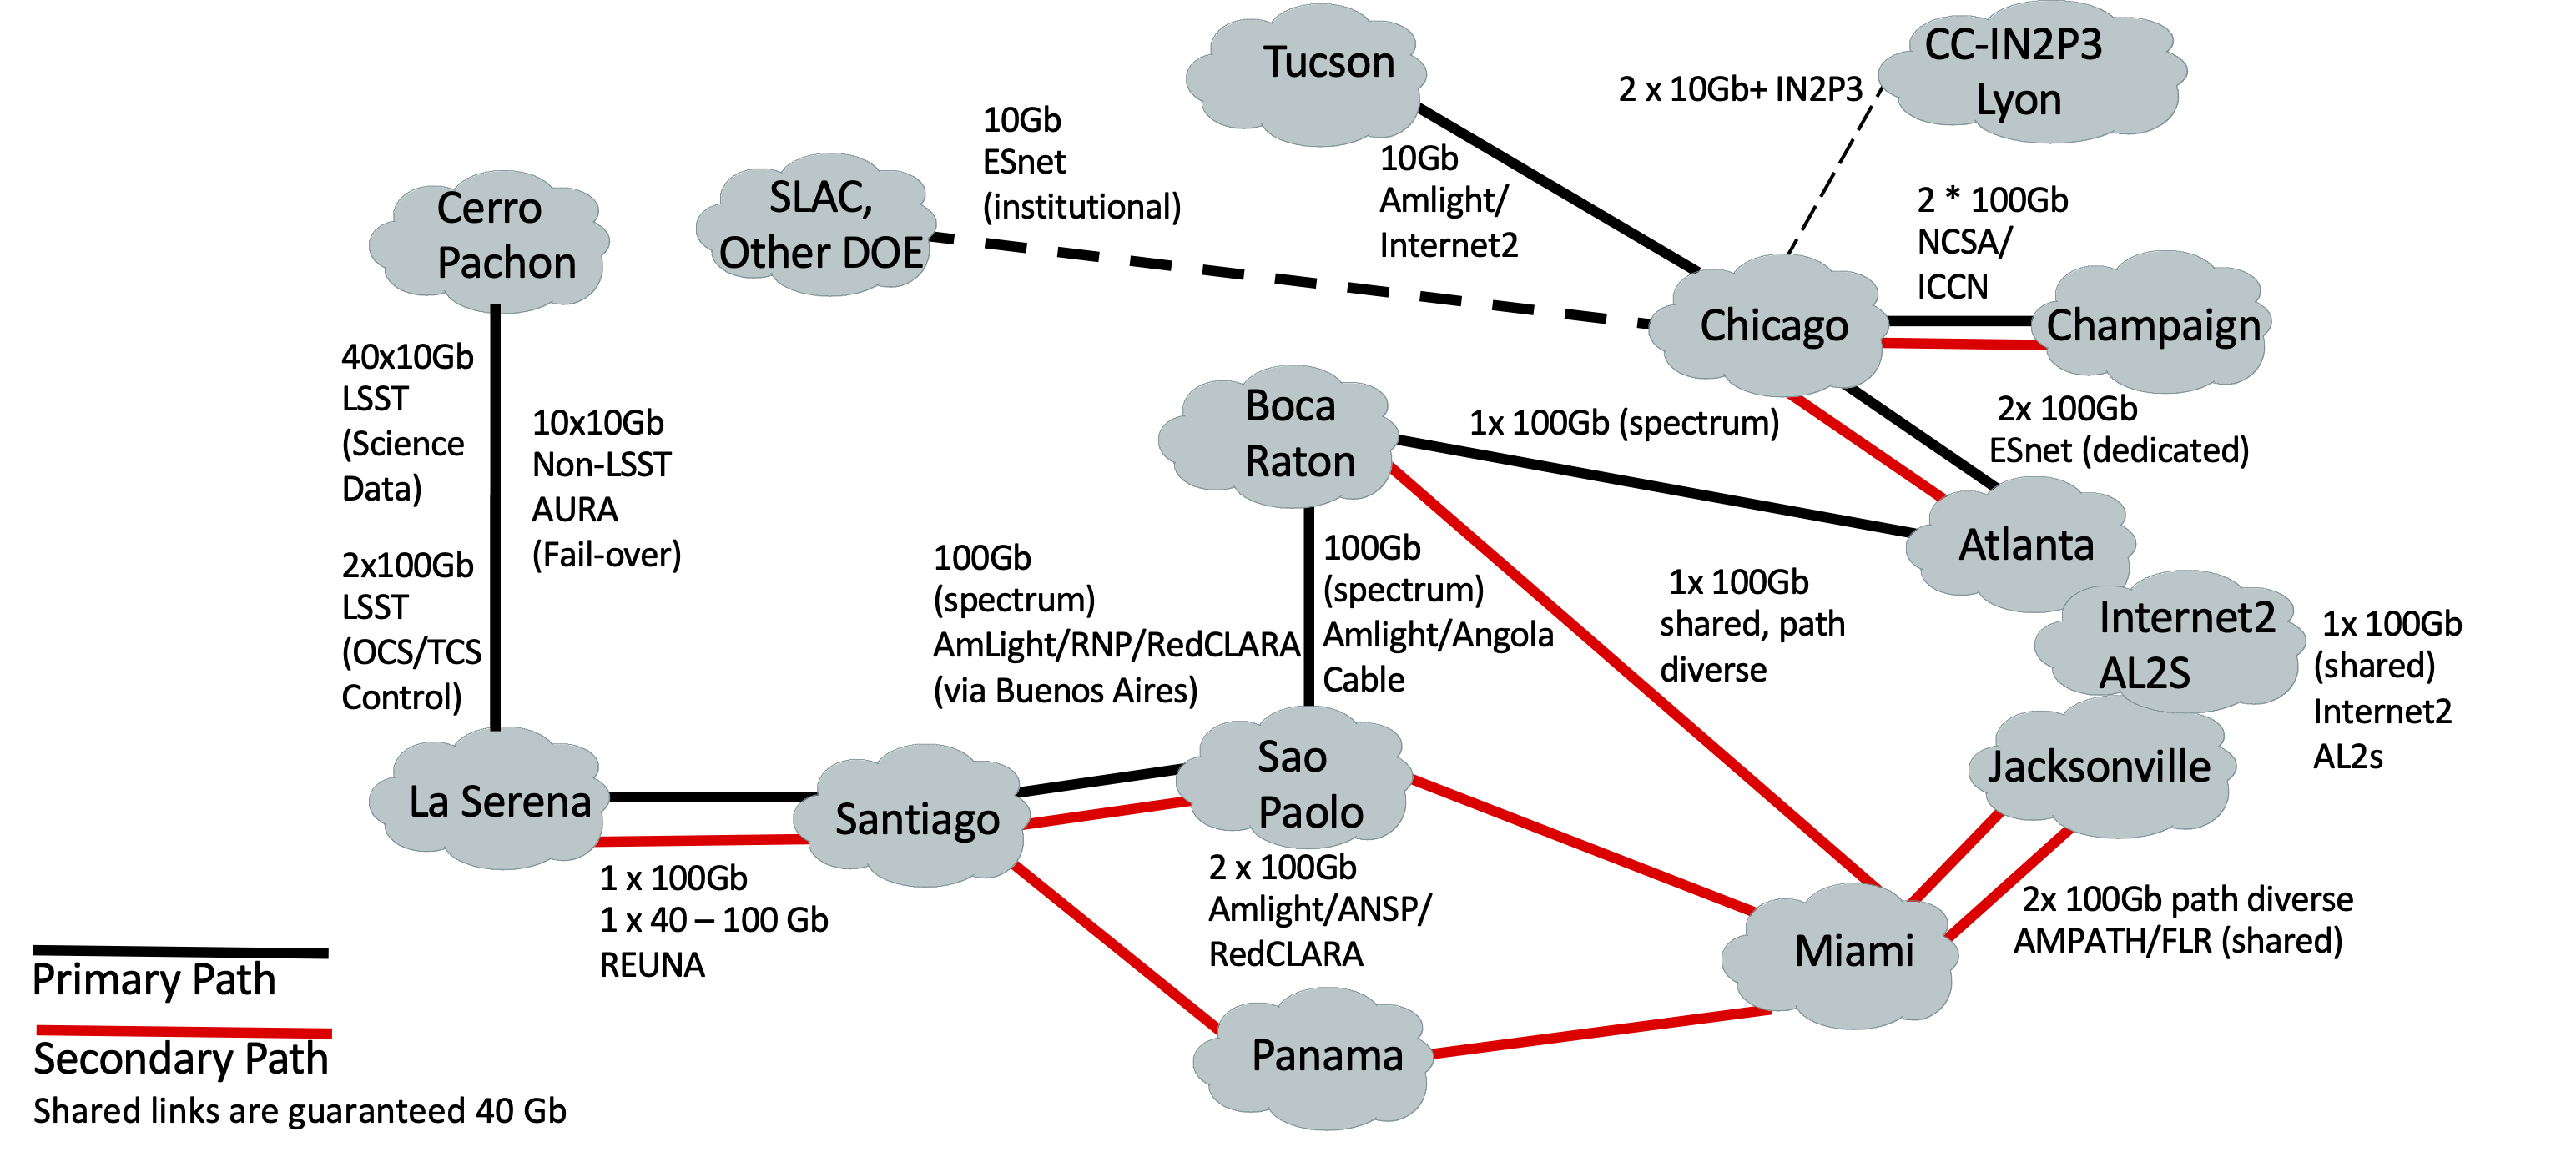
\includegraphics[width=1.0\textwidth]{NetworksFY22}
\caption{Rubin Observatory Network topology for FY22, the primary route is on dedicated lines, the back route is on shared equipment. Securing this beyond the level of the provider will be close to impossible.  \label{fig:net}}
\end{center}
% original https://docs.google.com/presentation/d/1wIN6Dj_rPn8TASBUkAm6_-Yh255Gz9VbwFi61t4LCFs/edit#slide=id.g55f7c0247e_0_2
\end{figure}


The transfers from Summit to Base and Base to NCSA go over private networks that are not part of the public Internet. We have our own dedicated fibers running from the mountain to the base \citedsp{LSE-78},
intercepting transfers would require physical access to the fibers - tapping those would probably disrupt our network at least temporarily.

We understand there is a concern for the transmission of the images for alert processing and
 \citeds{DMTN-163} covers this in detail.

 \rec{IT}{netsec}{IT shall purchase routers capable of performing AES\cite{aes} IPSec in between Chile and SLAC.}
{At lease two routers will be needed and we may need four for failover. This is a multi million dollar commitment. }

If we do not transfer embargoed images to France or UK we understand encryption on the international links should not be needed.



\section {Physical Security}

On the mountain and in the base facility Rubin networks and computers are in rooms requiring ID card access and the compounds have 24/7 security staff. We can increase physical security in Chile and SLAC.
Access from outside the site is only via VPN.
This also implies limiting the Rubin personnel who have access to the files during the night.


\rec{IT}{physsec}{IT shall increase physical security in Chile and SLAC.} {
Physical measures shall include :
\begin{itemize}
\item Locks on server racks.
\item Sensors and cameras to record the opening of cabinets.
\item Out of band channel for physical security alerts if main network is disabled.
\item Access control devices to server rooms that record entry/exit by personnel.
\item Auditable processes to handle on-boarding, off-boarding, maintenance work, removable media, etc.
\item For the secure delayed store :
	\begin{itemize}
	\item Controls to prevent booting from USB devices or copying to external media.
	\item Full disk encryption to protect against theft or returns of hardware.
	\end{itemize}
\end{itemize}

}

\subsection{Chile physical security} \label{sec:chileps}


\section{High level summary}\label{sec:sum}
Though the reason behind the call for security and the level required remain totally unclear
NSF and DOE asked for a brief summary of possibilities.
One should also consider which data we are talking about see \secref{sec:which}.
Items here are not costed but an indication is given in terms of low (possibly within cost), moderate (some \$100Ks), high (>\$1M)
Any change should be properly costed.


\begin{longtable}{p{0.75\textwidth} p{0.25\textwidth}}\hline
\textbf{Security idea} & \textbf{Rough cost level}  \\\hline
 {\bf Delay some or all images.} Depending on how secure this needs to be and where it is done the cost scales.  & Low to Moderate.\\
 {\bf Do alerts in Chile.} If we want to control image access for a longer period we could consider alert production in Chile. The hardware budget would remain the same but we may require extra support in Chile.  & Low to Moderate.\\
{\bf Encrypt all images.} This would have to be done on the summit or in la Serena before hitting the long haul network. Possibly no new hardware needed but a change in software.  & Can be Low \\
{\bf Transmission Layer Encryption.} Network encryption would probably require new hardware. & Moderate \\
{\bf Physically securing the network.} This will be next to impossible and would probably require new network agreements. This however would be the only way to ensure no packet snooping. & Very high \\
{\bf Avoid certain time coordinates.} This would require changing the scheduler to provide more constraints on pointing. &  Moderate  \\\hline
\end{longtable}

